\tikzset{every picture/.style={line width=0.75pt}} %set default line width to 0.75pt        

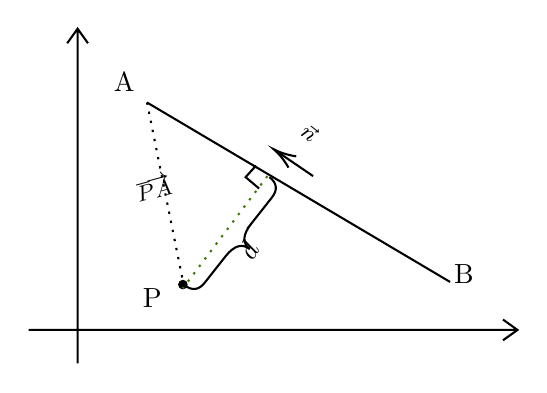
\begin{tikzpicture}[x=0.75pt,y=0.75pt,yscale=-1,xscale=1]
    %uncomment if require: \path (0,210); %set diagram left start at 0, and has height of 210

    %Shape: Axis 2D [id:dp44317292301248945] 
    \draw  (50,159.58) -- (285.5,159.58)(73.55,14.45) -- (73.55,175.7) (278.5,154.58) -- (285.5,159.58) -- (278.5,164.58) (68.55,21.45) -- (73.55,14.45) -- (78.55,21.45)  ;
    %Straight Lines [id:da2979242010824248] 
    \draw    (107,50) -- (253,136.45) ;
    %Shape: Circle [id:dp023999541748674025] 
    \draw  [fill={rgb, 255:red, 0; green, 0; blue, 0 }  ,fill opacity=1 ] (122.5,137.73) .. controls (122.5,136.75) and (123.29,135.95) .. (124.27,135.95) .. controls (125.25,135.95) and (126.05,136.75) .. (126.05,137.73) .. controls (126.05,138.71) and (125.25,139.5) .. (124.27,139.5) .. controls (123.29,139.5) and (122.5,138.71) .. (122.5,137.73) -- cycle ;
    %Straight Lines [id:da4396600304527325] 
    \draw    (187,85.45) -- (169.65,73.63) ;
    \draw [shift={(168,72.5)}, rotate = 34.28] [color={rgb, 255:red, 0; green, 0; blue, 0 }  ][line width=0.75]    (10.93,-3.29) .. controls (6.95,-1.4) and (3.31,-0.3) .. (0,0) .. controls (3.31,0.3) and (6.95,1.4) .. (10.93,3.29)   ;
    %Straight Lines [id:da11083812462923981] 
    \draw  [dash pattern={on 0.84pt off 2.51pt}]  (107,50) -- (124.27,135.95) ;
    %Straight Lines [id:da3033500048537672] 
    \draw [color={rgb, 255:red, 65; green, 117; blue, 5 }  ,draw opacity=1 ] [dash pattern={on 0.84pt off 2.51pt}]  (165,85.45) -- (124.27,139.5) ;
    %Shape: Brace [id:dp9223930624399752] 
    \draw   (125,137.95) .. controls (128.67,140.84) and (131.94,140.46) .. (134.83,136.79) -- (144.8,124.14) .. controls (148.93,118.91) and (152.83,117.73) .. (156.49,120.62) .. controls (152.83,117.73) and (153.06,113.67) .. (157.19,108.43)(155.33,110.79) -- (167.16,95.78) .. controls (170.05,92.11) and (169.66,88.84) .. (166,85.95) ;
    %Straight Lines [id:da5740957717017106] 
    \draw    (159.5,80.45) -- (154.5,85.95) -- (161,91.45) ;

    % Text Node
    \draw (89.5,34) node [anchor=north west][inner sep=0.75pt]   [align=left] {A};
    % Text Node
    \draw (253.5,126.5) node [anchor=north west][inner sep=0.75pt]   [align=left] {B};
    % Text Node
    \draw (103.5,138) node [anchor=north west][inner sep=0.75pt]   [align=left] {P};
    % Text Node
    \draw (184.96,57.48) node [anchor=north west][inner sep=0.75pt]  [font=\footnotesize,rotate=-38.36]  {$\vec{n}$};
    % Text Node
    \draw (147.97,122.08) node [anchor=north west][inner sep=0.75pt]  [rotate=-302.14]  {$d$};
    % Text Node
    \draw (98.59,87.74) node [anchor=north west][inner sep=0.75pt]  [font=\footnotesize,rotate=-344.6]  {$\overrightarrow{PA}$};


\end{tikzpicture}